\documentclass[english]{article}
\usepackage[utf8]{inputenc}
\usepackage[T1]{fontenc}
\usepackage{babel}
\usepackage{amsmath}
\usepackage{graphicx}
\usepackage{fancyhdr}
\newcommand{\scidatalogo}{
\includegraphics[height=24pt]{PiggyFinance_logo-iloveimg-cropped.png}}
\newcommand{\overleaflogo}{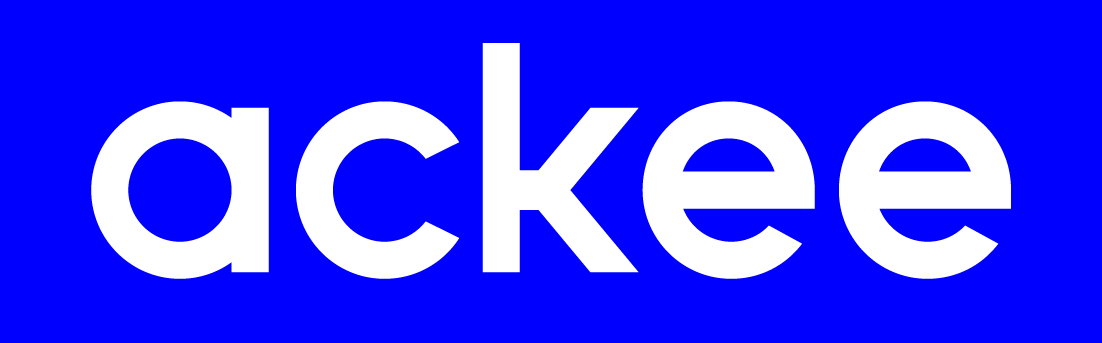
\includegraphics[height=24pt]{ackee_logo_rec_blue.png}}
\pagestyle{fancy}
\fancyhf{}
\renewcommand{\headrulewidth}{0pt}
\setlength{\headheight}{40pt} 
\lhead{\textsc{\scidatalogo}}
\rhead{\textsc{\overleaflogo}}
\usepackage{biblatex}
\addbibresource{main.bib}
\usepackage[toc,page]{appendix}

\begin{document}

\title{Draft: Piggy.finance}

\author{Dominik Veselý, Josef Gattermayer}

\maketitle
\thispagestyle{fancy}

\hfill
\hfill
\hfill

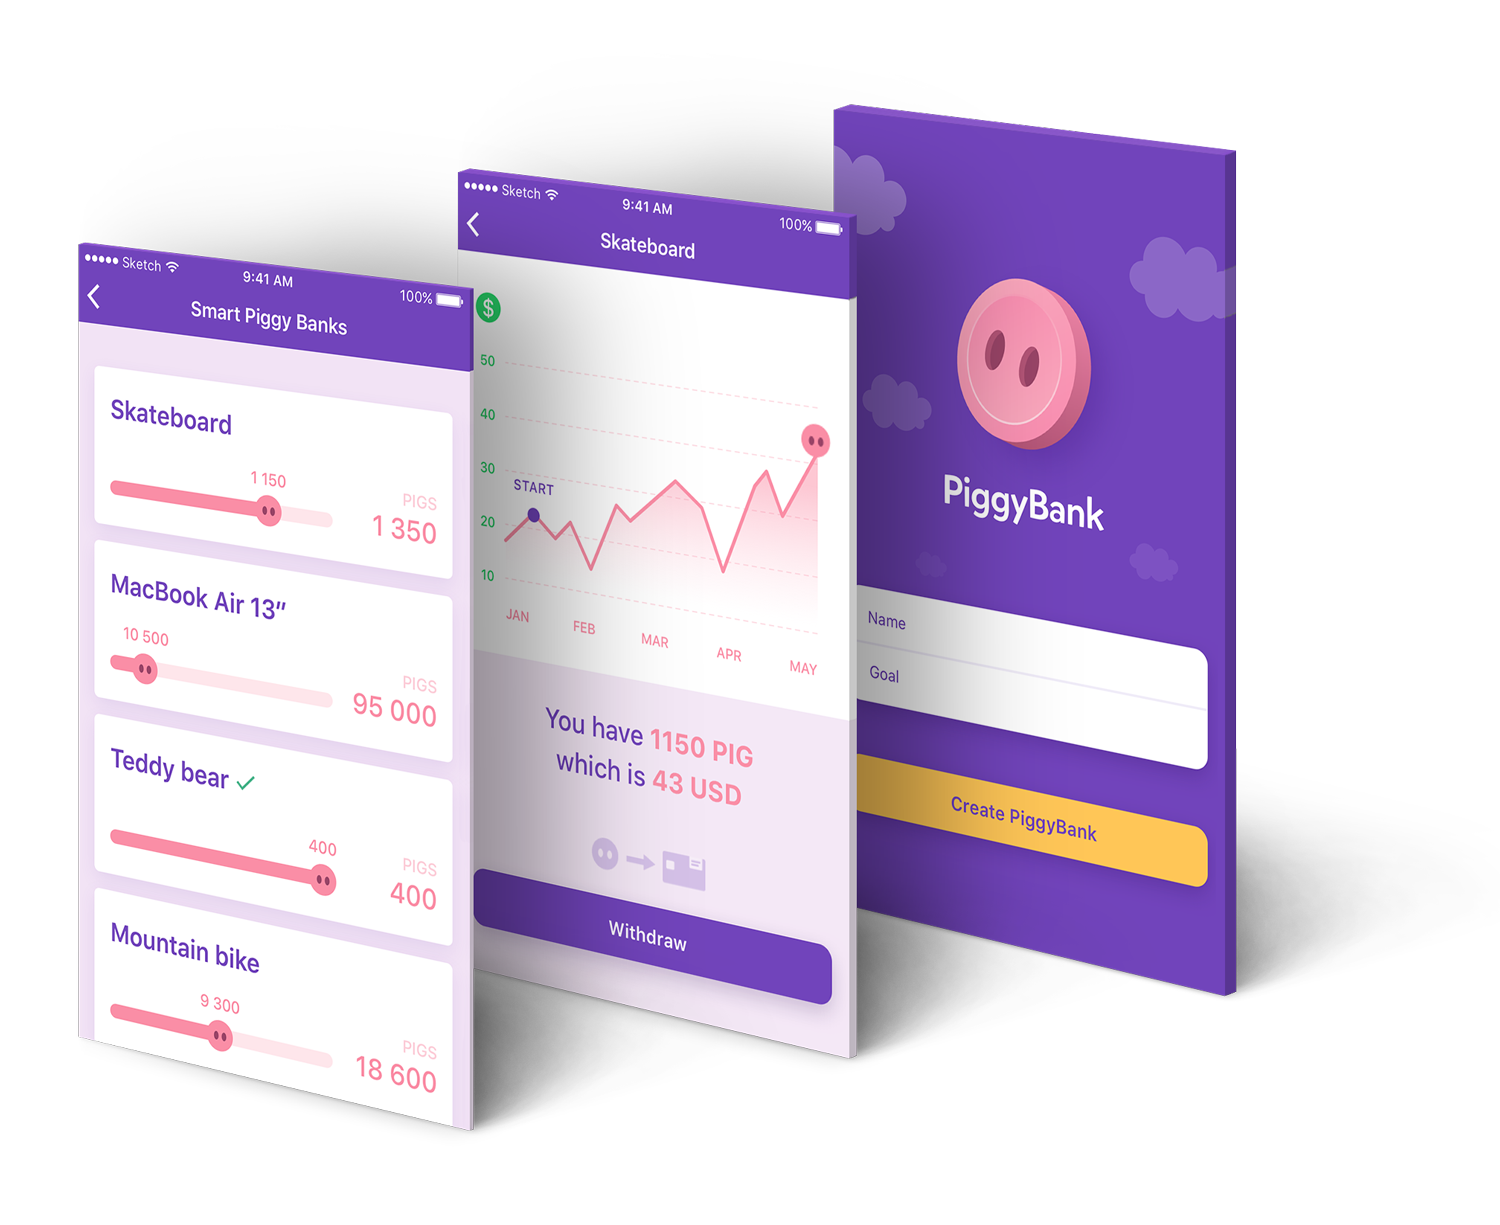
\includegraphics[scale=0.25]{Screeny.png}


\newpage
\tableofcontents
\newpage

\section{Executive Summary}

Cryptocurrencies have received significant attention in the last few years, and there is a good reason why. Many people see blockchain-based currency as the future of payment, and it is currently one of the best performing savings instruments. That being said, Ethereum smart contracts have introduced an even bigger toolset. Smart Contracts are a useful way of handing money operations such as making deposits, conditional payments, and more, without a centralized entity and having everything run in the Blockchain itself. We expect decentralised cryptocurrencies and smart contracts to become a regularly encountered procedure in everyday life.

Last decades in developed countries experienced very stable fiat currencies and have not witnessed phenomenons such as volatility, exponential growth of value, and extreme risk. This is what cryptocurrencies brought back. Only those who understand these terms can profit from cryptocurrencies, while others are at greater risk of experiencing huge losses.

Levels of financial literacy in the adult population are at a significant low. The OECD Recommendation \cite{oecd2016} underlines the importance of building such competencies early in life and ideally in schools.

That's what PiggyFinance is here for. It is a fully functioning decentralized mobile payment platform that, in addition tof its regular functions, teaches children and their parental counterparts about how to save money and understand volatility and currency exchange. It shows its users why decentralization is such a great thing. If there is a contract saying that children can empty their piggy banks after they have collected a specified amount, there needs to be a mutual trust between both children and parents that they will stand up to their promises. If such a contract is placed on a blockchain, there is no such authority, giving children the ability to withdraw money only when conditions are met without their parents being able to stop them. 

We aim to deliver an easy to use mobile platform for both children and parents where they can define money saving goals or pocket money withdrawal limits directly on a blockchain with no central authority present or programming required. In addition, we provide the full comfort of fiat payments using internationally accepted debit cards. 
Piggy.finance will be the cryptocurrency of the new generation. The current generation of crypto-adopters already have (or will have) children, and they will want a tool to teach their children about how to save money or, even better, how to work with cryptocurrencies. We will also directly educate children about cryptocurrencies at schools by providing and actively propagating our own cryptocurrency education course along with online courses and materials - all with PIG tokens playing the main role.

We present a realistic roadmap with a fully functioning product from the very first milestone that will be delivered in just 3 months time after a successful ICO. Unlike many other ICOs, we are already an experienced team with more than 40 programmers on board that have been delivering mobile solutions for top tech startups for the last 5 years.



\section{Problem Statement}

To define the need for a platform such as this one, we first need to take into account potential problems with the blockchain, smart contracts, and financial literacy. 

\subsection{Decentralization in Finance and Payments}

As seen in the case of Bitcoin (BTC), digital currency has taken the lead in establishing a new flow of resources that exist solely in  virtual space. Unlike the financial structures in place that lead to a centralized system, virtual currency utilizes blockchains to enable a flow of resources not dependent on a particular party.

The motivation behind decentralizing systems and not relying on banks and fiat currencies has been discussed several times in the past, and the current success of cryptocurrencies proves that there is a serious interest in utilizing this technology in real world affairs.

Nowadays however, cryptocurrencies are used mainly as an investment asset. The actual payment volume is still quite low and acceptance of cryptocurrencies in retail stores is still limited \cite{bitcoinaccpetance}. According to the Nilson Report \cite{NilsonReport}, payment cards are expected to increase from 21.3 percent to 21.93 billion by 2020. A hybrid model that introduces cryptocurrency investments but still offers fiat payments via payment cards seems like the ideal solution.

\subsection{Decentralized Apps and Payments within them}
Decentralized applications are pieces of software that execute and store results on a blockchain. These apps are tied together with currencies that allow parties to handle payments/deposits or actions without fear of interference. Once the deal is on the blockchain, whatever is written in the code commences without interference from any central authority. 
						
The launch of Ethereum in 2015 presented a new approach to building applications on blockchains. The new possibilities it offered brought smart contracts to the forefront of interest of influential companies such as Microsoft, ING, Toyota, Samsung, J.P. Morgan, State Street Corporation, Accenture, and Intel. Linked to Ether currency, the Ethereum network launched the Ethereum Virtual Machine (EVM), a distributed computing mechanism. In addition, the platform joined with Solidity, which granted it the possibility of writing exceptionally complex smart contracts within high level programming languages. As a result of Ethereum’s presence, the value of Ether currency has drastically increased by more than 3,400\%, ascending from its original position of under \$10 USD per ether to its current standing at an impressive \$300 USD per either since the end of September 2017.

Using smart Contracts on Ethereum has several key benefits:

\begin{itemize}
  \item Once contracts are deployed they don’t require interaction unless deemed necessary.
  \item Since EVM is a  turing complete machine, behaviour is deterministic. When you read the code, you will know exactly what will happen within the contract.
  \item Contracts are resistant to malicious attacks unless there are bugs in the code itself.
\end{itemize}

This of course has it own drawbacks. The greatest concern at the moment is  mass adoption, since many people outside of IT have begun buying cryptos  writing smart contracts in programming language might become a critical barrier. Another potential  problem is that even skilled programmers can run into bugs in their code and since codes are immutable on blockchains, this could lead to serious issues. Thus, it is necessary for us to find a way for regular people outside of IT as well as children to have access to smart contracts, and their usage should not be cumbersome. 

\subsection{Low financial Literacy}
According to the OECD/INFE International Survey of Adult Financial Literacy Competencies across the 30 participating countries and economies, just 51\% of the population achieved the minimum target score on financial behaviour \cite{oecd2016}, and here we are not even speaking of financial literacy in cryptocurrencies.

One of the key aspects of any cryptocurrency is its volatility. It is vital for people to understand this concept of volatile assets, and we are not speaking only about cryptos. A relatively stable period of financial assets in developed countries since the second world war has erased awareness about these terms. We think that now is the best time ever to educate children in financial literacy, Covering important topics such as saving money, understanding interest rates, the conversion between currencies, and the previously mentioned volatility. 

“Low levels of financial literacy (and in particular knowledge) in the adult population underline the importance of building such competencies early in life and ideally in schools” is the OECD’s recommendation \cite{oecd2016}.

\subsection{Market Size}
Our market will consist of two main groups - young relatives and friends of cryptocurrency users and cryptocurrency newcomers attracted by our Crypto to School program. 

\begin{itemize}
  \item There are between 2.9 million and 5.8 million users of cryptocurrencies \cite{cryptousers} who are considered more or less financially educated. We can assume they have or will have children, or know people who have children. We provide a tool that can easily be gifted, and can educate children on an extremely important field that classical education does not cover. 
  \item We also plan on attracting cryptocurrency newcomers. We will launch the Crypto to School education course where we create a complete education course, both for children and for teachers. This course will be offered to schools and our ambassadors will propagate it throughout schools worldwide.
\end{itemize}

Findings indicate that even children in developing countries, including poor ones, save \cite{callforsavings}. The demand for saving products in this age group is the largest, overperforming the demand for microcredits \cite{callforsavings}. Financial education is increasingly important, and not just for investors. It is becoming essential for the average family trying to decide on how to balance its budget, buy a home, fund its children’s education, and ensure an income when the parents retire \cite{oecd}. Those who understand the market gain a huge advantage - this pays especially for cryptocurrencies. Piggy.finance will be the entry cryptocurrency of the new generation.

\section{Solution Overview}

With the problem stated above, we have come to the conclusion that it is possible to solve all mentioned problems in one project. With the details described in the next chapters, we want to build a platform where children can be taught about crypto currencies which they will naturally use  later on in adulthood. This can be achieved through smart saving or pocket money distribution. As part of the project, there will be an educational program for children about crypto finances which will attract cryptocurrency newcomers to Piggy.finance.

\subsection{Development Platform and Currency}
For the reasons mentioned above, Ethereum is the platform of our choice. It has the widest adoption and good capabilities for writing smart contracts, which allows us to accomplish all our goals and bring the platform to life in the fastest time possible. 

The other big advantage of Ethereum is its ability to create sub-currencies, also known as tokens. We will create an asset called PIG which will be deployed as a smart contract conforming to the ERC20 standard for Ethereum crypto currencies, allowing the currency to be freely tradeable on the market. This token will be the only way how to fund a piggy.finance wallet. Money saving and money distribution will be done solely through  PIG tokens. Users who will want to withdraw will need to trade PIG for fiat currency. This guarantees ICO investors that there will always be enough tokens in a circulation.

\subsection{Open sourced Smart Contracts}
The main goal of the project is to create smart contracts that will act as piggy banks for children, with parents as supervisors. We want to create a special kind of Multi-signature wallet which will be deployed by the parent and enables children to save money until reaching specified amounts or distributing pocket money under specific circumstances. We plan on making smart contracts open sourced so that anyone can make changes to them and deploy them on their own. To simplify the functionality as stated in the beginning, we will create apps that will make the whole process of understanding smart contracts easier  for the users. The important thing is that the wallets will always work even without the app, just like with any other smart contract. 

\subsubsection{Smart Piggy Bank}
The Smart piggy bank contract is focused on saving, and acts as a saving smart contract wallet. It will teach children that they need to stick to their plan and that they are not able to withdraw from the Smart piggy bank until they have reached their desired amount. Upon deployment, the parent will specify:

\begin{itemize}
  \item The PIG token receiver’s wallet address. (i.e. child).
  \item The name of the Smart piggy bank. (i.e. Lego bank).
  \item The goal amount. (in PIGs).
\end{itemize}

Anyone can send PIG tokens to the Smart piggy bank to help reach the desired goal. Once the goal is reached, the child can withdraw PIG tokens from the piggy bank to their wallet. The contract will be written in such a way that will not allow the child to withdraw PIG tokens sooner, yet allowing the supervisor (parent) to withdraw PIG tokens from the Smart piggy bank any time for security reasons. In case of extreme volatility, the parent will be able to change the goal cap at any time. The idea behind this kind of saving is that the child can have multiple piggy banks for different purposes. This of course can also be very useful for adults or for group savings. 

\subsubsection{Smart Pocket Money}
The Smart pocket money contract is inspired by pocket money distribution. Let's say you want to give your children some money, but want them to spend it over a certain period of time and not all at once. The motivation behind this can be that you want to teach them responsibility, to set some ground rules, or to send money upfront so you don't have to think about it every week. As for the previous use case, the parent will deploy this contract and specify:

\begin{itemize}
  \item The PIG token withdrawal wallet address. (i.e. child).
  \item The amount that can be withdrawn during a period. (in PIGs).
  \item Period length (i.e 1 week).
  \item Overflow (i.e. if the amount is cumulatively raised throughout periods).
\end{itemize}

Again, anyone can send PIG tokens to the Smart pocket money contract but only the child can withdraw PIG tokens from the Smart pocket money, always fulfilling the permitted amount. If there is a situation when the PIG tokens are not withdrawn during a period and the overflow is set to true, the child can withdraw the PIG tokens for those periods. Once again, the parent will have access to this Smart pocket money at any time for security reasons. As for the previous contract, the parent can change the properties at any time. 

\subsubsection{Security Multi Signature Wallet}
In both previous use cases, money is withdrawn by the child to their Ethereum wallet. It’s well known that children lose things a lot. To prevent such stressful situations, it makes sense that even “ordinary” wallets should be supervised by parents. For this case, there will be an option to create a multi signature wallet. 

\subsection{Deposits, Withdrawals, and Payments}
We plan on attracting both current cryptocurrency users and cryptocurrency newcomers, therefore supporting deposits and withdrawals/payments in a fiat currency. In both cases however, the fiat currency will be traded for PIG tokens on the market.

\subsubsection{Deposit from fiat currency to PIG}
We will integrate a 3rd party service to allow easy fiat deposits. The 3rd party service will accept credit cards or bank wire transfers and will buy PIG tokens on the market. It will consequently raise the volume and demand of PIG tokens - we will never sell PIG tokens directly.

\subsubsection{Withdrawal / Payment with Fiat Currency}
The debit card will be represented in the app as a fiat wallet. We will emit Visa or Mastercard based debit cards in the main fiat currencies. Our debit cards will be accepted worldwide for payments and ATM withdrawals. There will be two steps: We will first emit debit cards by a partner 3rd party crypto debit card provider and secondly, as we obtain the MasterCard / Visa license, we will emit debit cards directly.

\subsection{Sustainable Funding}
The project must have sustainable funding in order to develop further and grow in value. The source of funding will be PIG exchanges to fiat a debit card where we keep a small fee from every transaction. The concrete value will not exceed 2\%. Out of this value we finance the platform and reward dividend holders in a 1:1 ratio.

\subsection{Dividends}
Dividends represent a passive income and will be implemented in piggy.finance for two reasons - education and stability. Each token holder can claim a dividend request - both the children and investors. We teach children about value growth and attract more long-term token holders rather than speculators. This will be the basis for a constant PIG token growth of value.

\subsection{Crypto to school education course}
We will reserve a considerable portion of the budget for creating an independent educational course. This course will cover financial literacy and cryptocurrencies. It will explain topics such as asset valuation, volatility, savings, dividends, and asset exchange. Materials will work with Piggy.finance, so we expect to attract cryptocurrency newcomers to the PIG token. This educational method was successfully used with the Ghana experiment that led to a significant increase in newly opened bank accounts.

We will develop courses for all 3 stages of education, with the addition of one online course. We will create materials for parents, teachers, and students. Our university ambassadors will provide support for teachers, and will be work alongside our advisors in offering the course across schools worldwide.

\subsection{Delivered Mobile Apps}
The success of this project lies in mass adoption, for which the key characteristic is simplicity. As will be mentioned below, we have 5 years of extensive experience with building startups, especially in the form of mobile & web apps. 

The most important thing is the mobile app. This will be a comfortable way of managing piggy banks and wallets by having control over their creation, checking balance, withdrawal functions, and transferable funds.

We plan on delivering one mobile app that will contain both roles: parents and children.

The basic list of functionality provided by the app: 

\begin{itemize}
  \item Creating wallets.
  \item Importing existing wallets.
   \item Grouping users (i.e. parent/child or group of friends).
   \item Creating piggy bank smart contracts.
   \item Creating pocket money smart contracts.
   \item List of your piggy banks and pocket money with progress and details.
   \item Child-comprehensive PIG to fiat currency exchange course graph.
   \item Option to send funds.
   \item Option to withdraw funds.
   \item Education course.
\end{itemize}

Apps will be created natively for Android and iOS for both phones and tablets using Kotlin and Swift languages.

\section{The Team}
Most newly found ICOs will face a common problem: “The Team.” They have an idea and often raise the required funds but then need to build a team that will work together - this takes months, sometimes years, even with almost unlimited resources. We have a team. Ackee is an established company from Prague, Czech Republic, with over 5 years of experience in building our own startups and delivering software for startups. The team has more than 40 programmers and designers ready to be focused on this project. Piggy.finance is founded by all 3 co-founders of Ackee.

\subsection{Founders}
The three co-founders already succeeded in building Ackee - a 50 person company which is growing every year. Each of the co-founders teaches at the CTU (Czech Technical University in Prague) \cite{cvutweb} - the best tech university in the Czech Republic \cite{cvut}.

Josef Gattermayer studied in the informatics Ph.D. program, and submitted his dissertation thesis on distributed systems this summer. As Chief Information Officer, he is responsible for infrastructure at Ackee. He is also a co-author of the Prague chip transport card Litacka \cite{litacka} that has been deployed to more than 800 000 users so far.

Dominik Veselý is a tech enthusiast and Chief Technology Officer at Ackee. At the CTU in Prague, he is a speaker for the  iOS development course and leads a number of master theses. He is also often a speaker at tech events such as mDevCamp \cite{mdevcamp}.

Martin Půlpitel is CEO at Ackee and an assistant professor at the CTU in Prague. He is a 
guarantor and speaker of a project management course. He is also an author of the leading Czech mobile development conference mDevTalk \cite{mdevtalk}. Martin has two children and wants them to receive the best education.

\subsection{Related Experiences}
We have extensive experience in the fields of education and technologies. As teachers we know how important is to create quality study materials, and s programmers we know how to build quality software products. We have built more than 20 startups from the ground up and a total of more than 100 other IT projects. 

We develop and co-own another child focused startup babysitting.today, which is a shared economy service that pairs children with babysitters. And we own 100\% shares in a profitable startup App4Fest which has been on the market for 4 years.

Among with work for startups, we have worked on projects for big brands such as T-Mobile, Skoda Auto, and Deloitte. 

\subsubsection{Related Research}
Ackee focuses on researching distributed reputation systems. This research is based on a dissertation thesis by Josef Gattermayer, Ackee’s co-founder. The dissertation thesis dealt with the reputation of single nodes of a peer-to-peer non-dedicated distributed computation cluster and single results were presented as academic papers on scientific conferences such as IPDPS \cite{ipdps}, PDP \cite{pdp}, and ICPP \cite{icpp}. It solves the open multi agent system problem \cite{multiagent} through blockchain technology. The current aim is to make this a general solution for a variety of use cases. We see a huge potential in this area as almost every ICO will need to deal with this topic. Our work in progress can be found at \cite{ackeenetwork}.

\section{Technical Overview}
The greatest value of the PiggyFinance platform is to offer the easiest way possible for working with cryptocurrency and using our smart contracts. The platform will provide an easy to use interface in a form every user knows: a simple mobile app. Via this interface, users can deploy our precisely written, tested, and security checked smart contracts for withdrawing PIG tokens to fiat currency in the same fashion they use their mobile apps on day to day basis. This seamless integration of blockchain and traditional technologies will let users work with simplicity without even knowing that they just deployed a code into a blockchain. 

Users will deploy contracts themselves (with or without the app) with their public & private key, so PiggyFinance will not have any control over it.


Because the PiggyFinance platform won't be storing any of its users tokens (users will store them in their deployed contracts), there is no need to worry about attacks on the platform or users losing money. 

Security is still a big concern of ours, and we will make sure that all of our Smart Contracts are audited and security checked by our advisors. Since contracts will be open sourced, the community will be able to let us know about any bug they find, making it possible for us to fix or enhance it. Through this transparency, users will not need to worry about the safety of their money.

Speaking of deployed contracts, we are aware of the fact that deploying contracts costs lots of gas and therefore money for our users. Since security is our biggest priority, we need to let users deploy contracts on their own, but we will implement contracts and deploy mechanics that are as efficient as possible. 

We will achieve this by using Ethereum’s features and programming styles. We plan on utilizing a technique known as Call Forwarding, which allows us to deploy one contract as a Library, and the deployed contract forwards the execution on this Library.

Executing transactions is another thing that we need to deal with. Since we let users deploy contracts on their own, withdrawing and sending funds on Ethereum costs GAS. Children and parents will therefore need Ethereum in their wallets. In terms of money, this is not a problem because the standard cost of gas for transferring is only around \$0.023. We will make the process of acquiring ETH for PIG transactions transparent to the end user, see Figure \ref{fig:piggy-diagram}.

We will trade needed ETH (gas) with users’ PIGs on background via services such as ShapeShift. Users will still be able to fund their wallet by ETH if they would like to, we just understand that bringing another currency can be confusing for some users. We will discuss ETH and GAS in our educational materials, so people understand that decentralization and sending funds needs to have some kind of fee just like regular banking.

\begin{figure}[h]
    \centering
    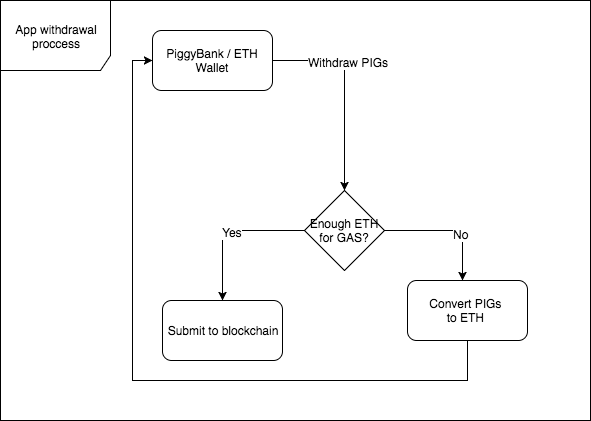
\includegraphics[width=1\textwidth]{PiggyBank-Diagram.png}
    \caption{Gas payment process}
    \label{fig:piggy-diagram}
\end{figure}

\subsection{ATM Withdrawals / merchant payments}
Initially, the operations of the fiat currency will be done by a partner 3rd party crypto debit card provider to speed up the launch process. In this case the fiat account will be managed by the partner and we will provide a user interface in the app for the account. This is a rapidly developing area and conditions change quickly so we are not planning on staying vendor-locked with one partner, but to choose a partner with the best conditions for the time being. We will however always provide the same user interface to the user in the app. The process illustrates Figure \ref{fig:piggy-diagram2}.

\begin{figure}[h]
    \centering
    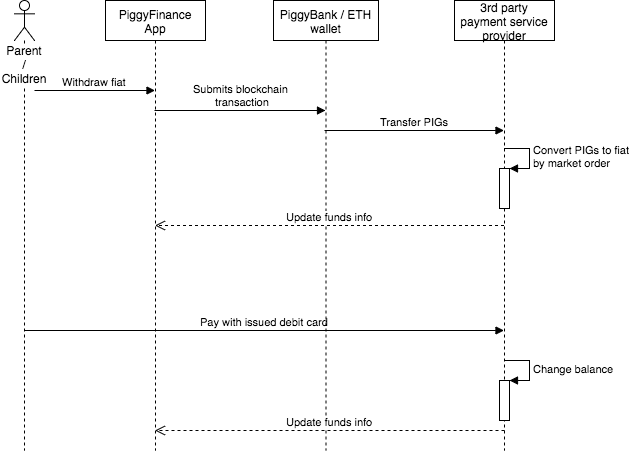
\includegraphics[width=1\textwidth]{PiggyBank-Diagram2.png}
    \caption{Withdrawal process with a 3rd party provider}
    \label{fig:piggy-diagram2}
\end{figure}

In the next step we will cover more operations by ourselves and emit cards directly with a banking partner. We will also manage PIG to fiat conversions through an exchange partner. The process illustrates Figure \ref{fig:piggy-diagram3}.

\begin{figure}[h]
    \centering
    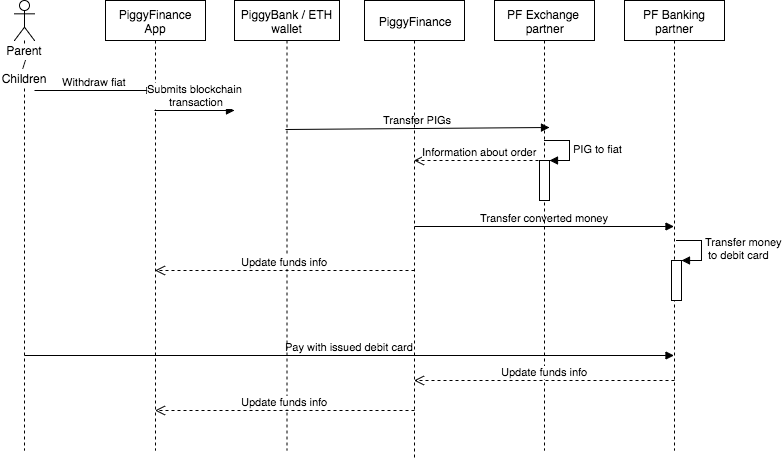
\includegraphics[width=1\textwidth]{PiggyBank-Diagram3.png}
    \caption{Withdrawal process handled by Piggy.finance}
    \label{fig:piggy-diagram2}
\end{figure}

\subsection{Dividend distribution}
Dividend distribution is a challenge on Ethereum, but as stated in the previous chapter, interest rate earnings are a crucial part of the whole economy. On Ethereum there is a common pattern of rewards based on PoW. We will be rewarding token holders that actively claim their dividend request. The concept will be based on claiming periods. During each period (i.e 1 month), all dividend incomes are summed up to be divided. All token holders will be able to claim their portion based on the amount of tokens they hold and the time that they hold them. After the claiming period ends, holders can withdraw their portion of dividends.

%\subsection{State Diagrams}

\section{Deliverables and Roadmap}

The project will be divided into 3 milestones, piggy.finance being a fully working platform in every milestone. The difference is in the amount of resources we put on boosting the piggy.finance user base.

\subsection{Milestones}
\subsubsection{Smart contract and apps - 1st Milestone}
This milestone delivers basic functionality. We will deploy smart contracts to the Ethereum blockchain and open source their code. We will make Android and iOS apps available on platform stores or a free download. The apps will contain all the described functions except the fiat wallet and debit card payments.

\subsubsection{Fiat payments by debit card - 2nd Milestone}
On top of milestone 1 we will also introduce the fiat wallet in the app and will connect this wallet to a worldwide acceptable debit card.

\subsubsection{Crypto to school education course - 3rd Milestone}
We will deliver materials for the education course and our ambassadors will actively find and support schools that agree to include this program in their lectures.

TODO: GANT chart
TODO: graph representation
TODO: market cap

\section{ICO and Token mechanics}
The ICO will start on 6.11.2017 and will end on 6.1.2018. It will be determined by the start and end block, so precise times may vary depending on mining speed. There is no predetermined supply of PIG tokens before ICO, so everything depends on demand. The price of PIG tokens will be determined by Ethereum since the whole platform relies on it. 1 ETH = 150 000 PIGs, which will be a fixed price during the ICO.

There will be a minimum cap and hard cap for the ICO. If the minimum cap will not be reached, the invested ETH will automatically be transferred back to the sending wallet after the end of the sale. 

There will be three cap goals and by reaching each of them, we will deliver a specified milestone. Ethereum raised between goals will be used for marketing and platform improvements.

\begin{itemize}
  \item The minimum cap will be set to 1500 ETH, which is the price needed to create the first milestone and is the minimum product of the platform. 
  \item The second goal will be set to 5000 ETH.
   \item The third goal will be set to 15000 ETH.
\end{itemize}

Ethereum raised for milestone 1 will be released immediately to fund the development. After delivery of milestone 1, we will release resources for the development of milestone 2. The same way resources for milestone 3 will be delivered no sooner than milestone 2 is delivered to the app stores.

There will also be a hidden hard cap which will be disclosed once reached. We don't want to collect more money than needed. The hard cap will be hashed and hash will be on our website and ICO contract. If the hard cap will be reached, we will stop the token sale and disclose the hash. 

\subsection{Distribution Structure}
Since we will sell an upfront unknown umount of PIG tokens for a fixed price per token, the total amount of minted PIG tokens will depend on demand. The total supply will consist of tokens sold during the ICO and an additional 30\% minted for team members and advisors. Those will be the only tokens ever minted. Tokens for advisors and team members will be locked for a period of 6 months and 1 year, so that the piggy.finance team won't be able to manipulate them. Thus, or one year, all tokens in circulation will only be those sold during the ICO in the hands of community.

\begin{itemize}
  \item 60\% of tokens will be sold during the ICO.
  \item 20\% of tokens will be reserved for the Piggy.finance team.
  \item 10\% of tokens will be reserved for Pigg.finance advisors.
  \item 10\% of tokens will be reserved for promotion.
\end{itemize}

\section{Legal Considerations}
TODO

\printbibliography

\newpage

\begin{appendices}
\section{State Diagrams}

\begin{figure}[h]
    \centering
    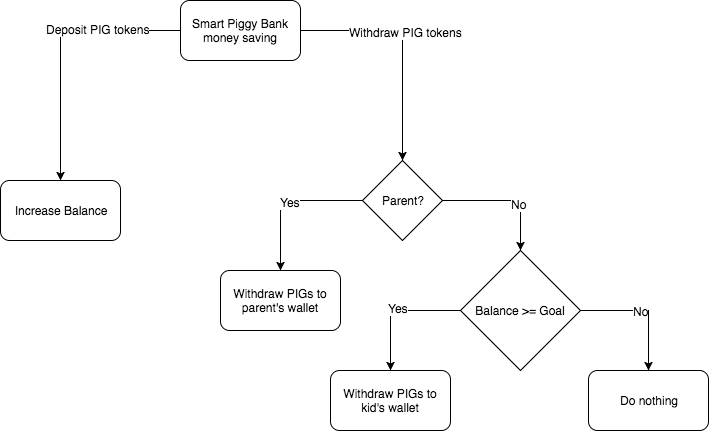
\includegraphics[width=1\textwidth]{PiggyBank-StateDiagram1.png}
    \caption{Smart Piggy Bank}
    \label{fig:piggy-diagram}
\end{figure}

\begin{figure}[h]
    \centering
    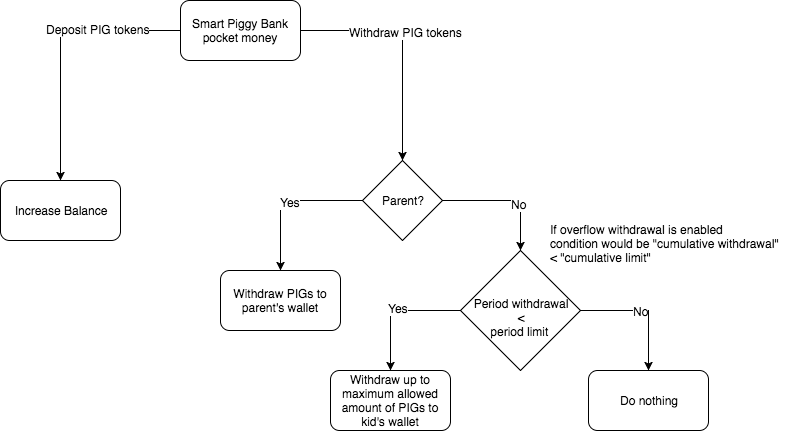
\includegraphics[width=1\textwidth]{PiggyBank-StateDiagram2.png}
    \caption{Smart Pocket Money}
    \label{fig:piggy-diagram}
\end{figure}

\end{appendices}

\end{document}